%
% This is Chapter 1 file (chap1.tex)
%
\chapter{Introduction}
This is the information for the first chapter, Chapter 1.  Copy the base file, chap1.tex, for additional chapter needed such as chap2.tex, chap3.tex, etc. Modify the main base file to include each additional chapter file.

\section{intro}
This is the information for the first section of the first chapter.

\subsection{intro2}
This is the information for the first section of the first chapter.

\subsubsection{intro3}
This is the information for the first section of the first chapter.

\subsection{intro4}
This is the information for the first section of the first chapter.

\subsubsection*{intro5}
This is the information for the first section of the first chapter.

\section*{intro6}
This is the information for the first section of the first chapter.

\begin{table}
\begin{center}
\renewcommand{\arraystretch}{2}
\begin{tabular}{c|c}\hline
\multicolumn{2}{c}{All elements}\\
\hline
1$^{st}$ & 2$^{nd}$\\\hline
1 & 2\\
3 & 4\\\hline
\end{tabular}
\renewcommand{\arraystretch}{1}
\end{center}
\caption{Table Example}
\end{table}

\newpage

\begin{figure}
\begin{minipage}[b]{2.65in}
\begin{center}
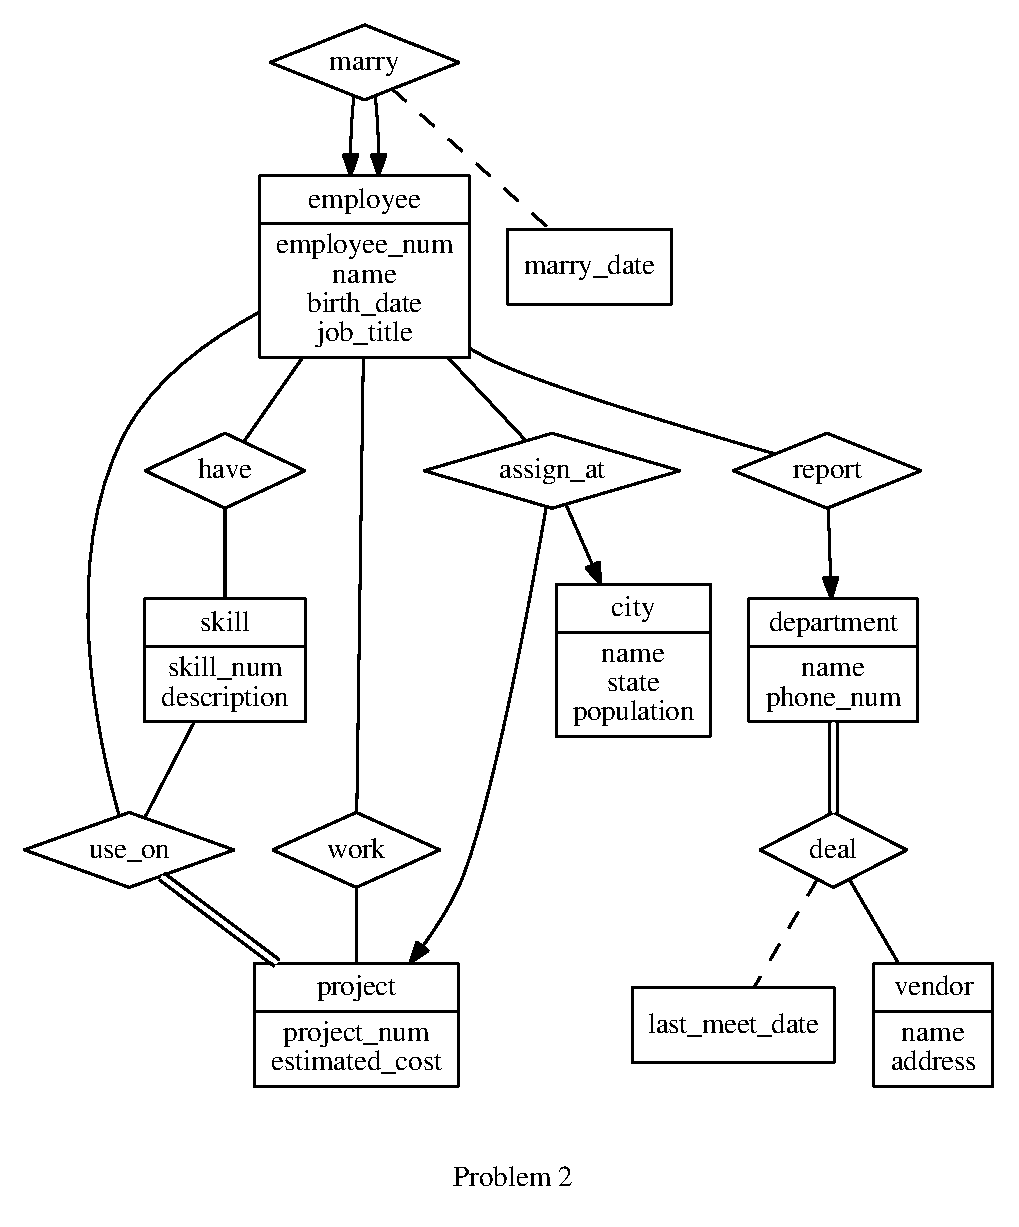
\includegraphics[width=2.85in]{ant}
\\hello
\end{center}
\end{minipage}
\hspace*{.375in}
\begin{minipage}[b]{2.65in}
\begin{center}
\includegraphics[width=2.85in]{search-page}
\\world
\end{center}
\end{minipage}
\caption{Figure Example}
\end{figure}

\begin{figure}
\begin{algorithmic}[1]
\Procedure{Euclid}{$a,b$}\Comment{The g.c.d. of a and b}
\State $r \gets a\bmod b$
\While{$r\not=0$}
\State $a\gets b$
\State $b\gets r$
\State $r\gets a\bmod b$
\EndWhile
\State \textbf{return} $b$
\EndProcedure
\end{algorithmic}
\caption{Euclid’s algorithm}
\end{figure}


One of my chapter headings\cite{ddd} is \cite{fff} at the bottom of a page and I'd like to drop it down to start off the next page. Any suggestions would be much appreciated.
$$ a+\pi^2 \ $$

